%#####################################################################
\chapter{ns-3によるOpenFlowネットワーク構築}
%#####################################################################

 本節では,現在愛媛大学が採用しているEUNETについて説明し、今回の研究で提案するOpenFlowを用いたネットワークモデルの構築法について説明する。

\section{EUNET}

現在、愛媛大学ではEUNETと呼ばれるネットワークが稼働している。
EUNETは大きく分けると、キャンパス内を網羅するエッジネットワークと、愛媛大学の城北、重信、樽味、持田の各キャンパスとデータセンタを接続するL3サブネットの二種類がある。

EUNET全体で現時点で約700ものネットワーク機器が存在し、今後も増えると考えられる。

\subsubsection{L3サブネット}

EUNETの中心部に位置するネットワーク。
愛媛大学の各キャンパス及びデータセンタに設置されているコアスイッチ群、以下に説明するスーパーコアから構成され、愛媛大学の各キャンパス間の接続およびインターネットとの接続を行う。

\subsubsection{スーパーコア}

L3サブネットの中核を成すネットワーク機器群。
EUNETとインターネットとの接続点に設置されており、ファイアウォール、検疫ゲートウェイ、侵入防止システム(IPS)、セキュアゲートウェイの機能を持ち、EUNETに悪影響を与える可能性のある通信について対応する機能を備える。
インターネットなど外部との接続の場合のみならず、EUNET内部でも異なるセグメント間の通信は、必ずスーパーコアを通るような設計になっており、ネットワーク内部の脅威にも対応することが可能である。

しかし、現在のスーパーコアの設計は、異なるセグメント間の通信をIPSに通す際に、図 \ref{fig:3-0}のような特殊な経路選択をしている。

\begin{figure}[tb]
\begin{center}
\scalebox{0.5}{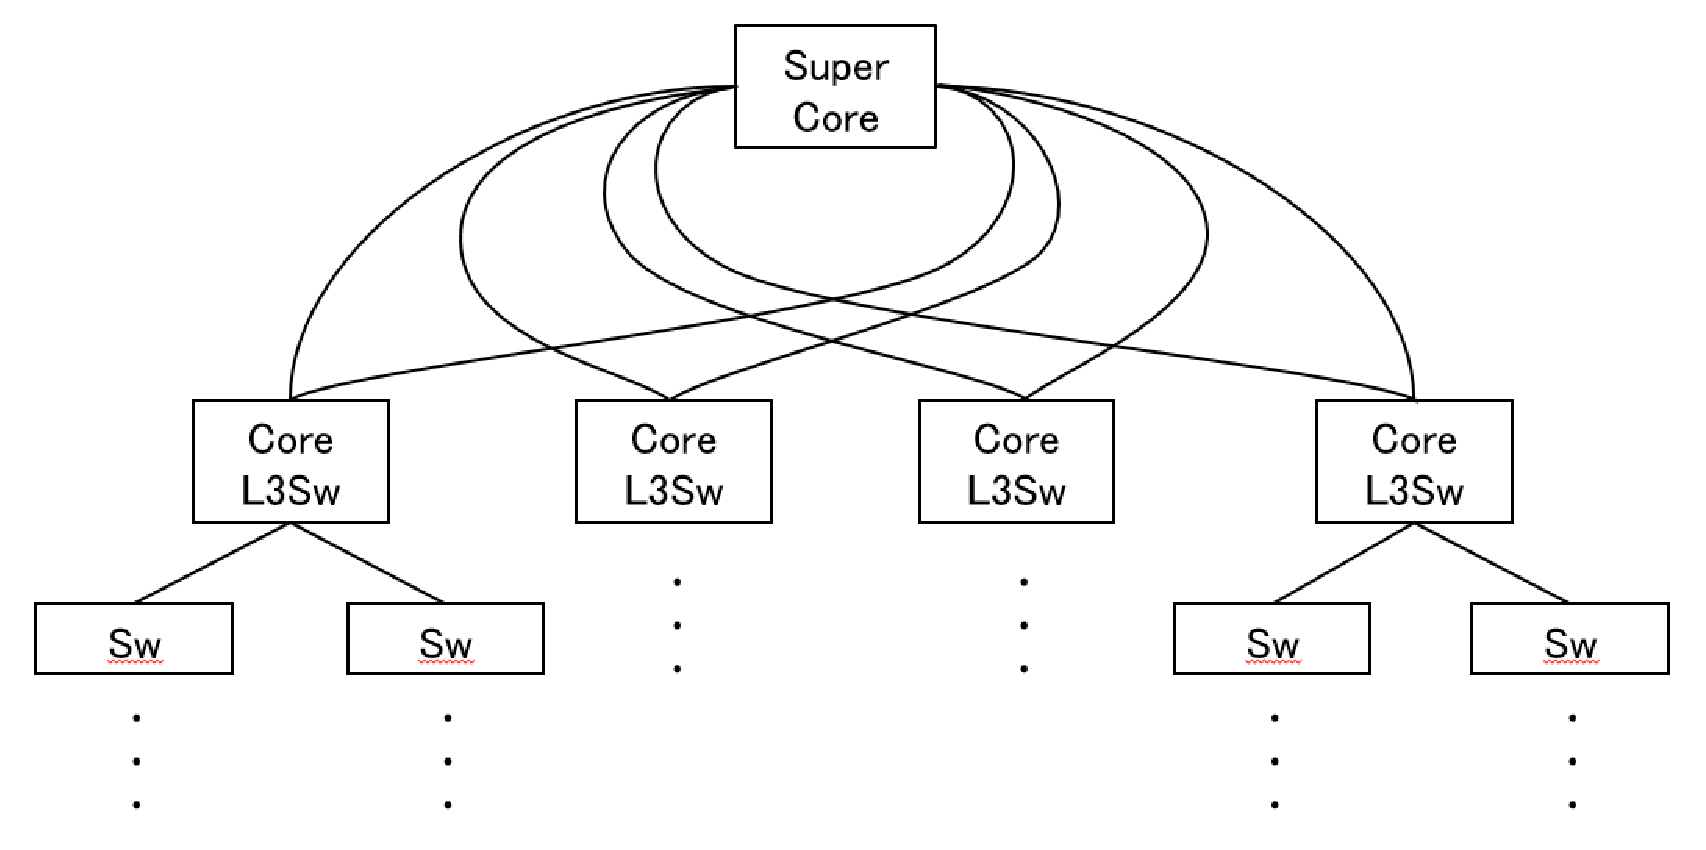
\includegraphics{./img/eps/3-0.eps}} 
\caption{現在のスーパーコアの設計}
\label{fig:3-0}
\end{center}
\end{figure}

一般的な通信は、任意の2つのホスト間のパケットの経路は往復ともに同じであるという対称な通信を行っているが、現在導入されているIPSは、パケットの入力ポートおよび出力ポートを明確に設定することで、パケットの経路は対称でない。
このようなパケット通信は一般的なIPSでは正常に動作せず、限られた一部のIPSでしか動作しない。

\section{ネットワークモデル構築法}

本節では、上記の問題点があるスーパーコアを改善したネットワークモデルを構築する方法を説明する。

スイッチをOpenFlow対応スイッチへと変更してネットワークを構成し、2種類のOpenFlowコントローラによってスイッチを制御することで、以下の図 \ref{fig:3-1}のようなネットワークを構築する。
OpenFlowスイッチは、2種類のOpenFlowコントローラによって制御を行う。

\begin{figure}[tb]
\begin{center}
\scalebox{0.5}{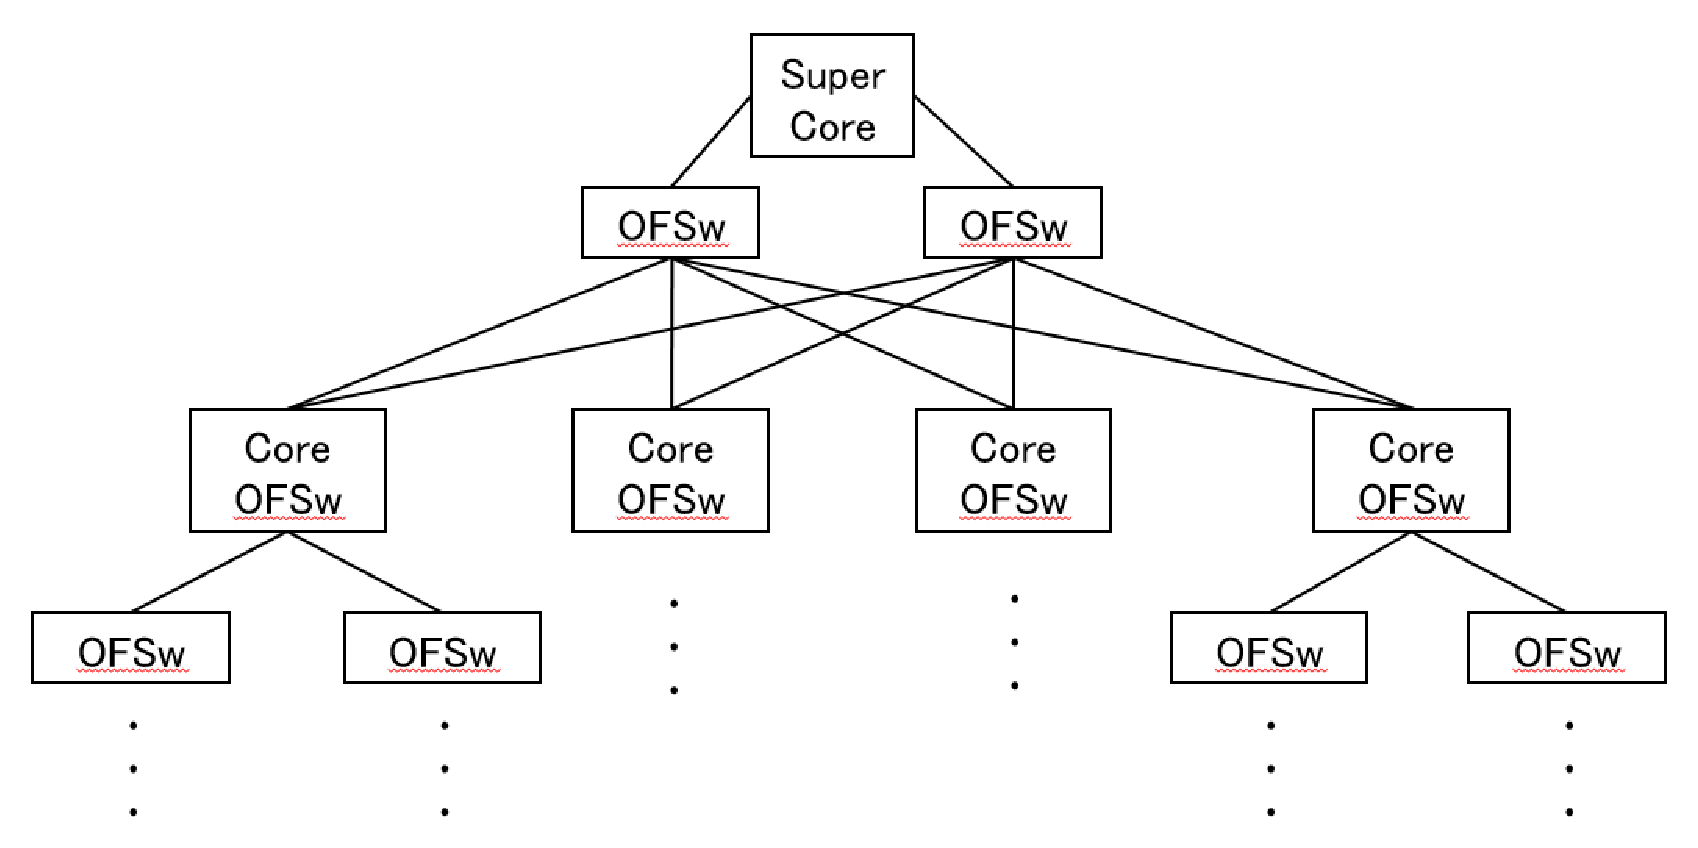
\includegraphics{./img/eps/3-1.eps}} 
\caption{提案するネットワークモデル}
\label{fig:3-1}
\end{center}
\end{figure}

次に、スイッチを制御する2種類のOpenFlowコントローラについて説明する。

\subsubsection{BasicController}

BasicControllerは、コアスイッチより下層に位置するスイッチ全て、および従来のIPSとコアスイッチの間に新たに設置するスイッチを制御するOpenFlowコントローラである。
所属するOpenFlowスイッチは、物理ポートの1つを上層のネットワークと接続し、それ以外の物理ポートを下層のネットワークおよびホストと接続させることが必要。

下層のネットワークおよびホストから入力されたパケットを無条件で上層のネットワークへと出力し、上層のネットワークから入力されたパケットは、ルーティング規則に従い下層のネットワークおよびホストへと出力するという処理を行う。

\subsubsection{CoreSwitchController}

CoreSwitchControllerは、コアスイッチを制御するOpenFlowコントローラである。
コアスイッチは、物理ポート2つをIPSとコアスイッチの間に新たに設置するスイッチ2つにそれぞれ接続し、それ以外の物理ポートを下層のネットワークと接続させることが必要。

下層のネットワークから入力されたパケットは、上層のネットワークへ出力する際に、MACアドレスの比較を用いて出力する物理ポートを決定する。
パケットから送信元MACアドレスと宛先MACアドレスを取り出し、送信元MACアドレスの方が小さい場合は物理ポート0から、大きい場合は物理ポート1から出力するように処理を行う。
MACアドレスは各ネットワーク機器に対して、唯一かつ一意に割り振られているため、通信を行う任意のホスト2台間の通信経路は一意に決定される。

上層のネットワークから入力されたパケットは、ルーティング規則に従い出力ポートを決定する。
このとき、上層のネットワークに出力しないように設定する必要がある。